\documentclass[a4paper, 12pt]{article}
% Pacotes
%%% fontes %%%
\usepackage[T1]{fontenc}
\usepackage{ucs}
\usepackage[brazil]{babel}       % hifenaçao
\usepackage[utf8x]{inputenc}     % acentuação
\usepackage{ae,aecompl}  % pdfs mais bonitos =)
\usepackage{multirow}

\usepackage{epsfig}
\usepackage{paralist} 
% Links
\usepackage[linkbordercolor={1 1 1},urlcolor=black,colorlinks=false]{hyperref}
\usepackage{amsmath,amsfonts} % matematicos
\usepackage{amssymb}
\usepackage{enumerate} % enumeração
\usepackage{indentfirst} % retira padrão americano de parágrafos
\usepackage{pslatex}
\usepackage{verbatim}
\usepackage[left=1.5cm,right=1.5cm,top=2.0cm,bottom=2cm]{geometry}
\usepackage{graphicx}
\usepackage{epstopdf}
\usepackage{multicol}
\usepackage{mdframed}
\usepackage{algorithm}
\usepackage{listings}
\usepackage[noend]{algpseudocode}
\lstset{language=C}
% Declarations
%\newcommand{\card}[1]        {\left|#1\right|}
\setlength{\columnsep}{30pt}
\setdefaultleftmargin{3em}{}{}{}{}{}
\newcommand{\BOX}[2]{\framebox[#1cm]{\rule{0mm}{#2cm}}}
\newcommand{\paritem}{\par \item}
\newcommand{\datasuper}[1]{${}^{\mbox{\underline{\scriptsize{#1}}}}$ }
\newcommand{\lfrac}[2]{\Large\(\frac{#1}{#2}\)\normalsize}
\newenvironment{subitens}{\begin{inparaenum}[\bfseries{(}a)]}
 %\setlength{\parindent}{-4em}}
 {\end{inparaenum}}

\newenvironment{exercicios}{\begin{enumerate}
 \renewcommand{\theenumi}{\textbf{\arabic{enumi}.}}
 \renewcommand{\labelenumi}{\theenumi}}
 {\end{enumerate}}

% Declarations
\setlength{\columnsep}{30pt}
\setdefaultleftmargin{3em}{}{}{}{}{}

\begin{document}

\begin{titlepage}
\begin{center}

% Upper part of the page. The '~' is needed because \\
% only works if a paragraph has started.

\includegraphics[width=0.4\textwidth]{./logo.jpg}~\\[2cm]

\textsc{\LARGE Universidade Estadual de Campinas}\\[1.5cm]
\textsc{\Large MC613 - Laboratório de Circuitos Digitais}\\[0.5cm]

% Title
\rule{\linewidth}{0.5mm} \\[0.4cm]
{ \huge \bfseries Relatório do Projeto - Gerador de Fractal \\[0.4cm] }

\rule{\linewidth}{0.5mm} \\[1.5cm]


% Author and supervisor
\noindent
\begin{minipage}{0.4\textwidth}
\begin{flushleft} \large
\emph{Autor:}\\
Matheus  \textsc{Jun Ota} \\
Alana  \textsc{Idalgo}
\end{flushleft}
\end{minipage}%
\begin{minipage}{0.4\textwidth}
\begin{flushright} \large
\emph{RA:} \\
138889\\
145166
\end{flushright}
\end{minipage}


\vfill

% Bottom of the page
{\large \today}

\end{center}
\end{titlepage}

\section{Teoria}

O conjunto de Mandelbrot(criado por Benoît Mandelbrot) pode ser definido como todo ponto c tal que a seguinte sequência não tenda ao infinito:
$$ z_0 = 0$$
$$z_{n+1} = {z_n}^2 + c$$

onde $z_{n+1}, z_n, c ∈ C$

Uma das propriedades do conjunto de Mandelbrot é que ele está contido num disco centrado na origem e de raio 2. Portanto, considerando a tela de um monitor como o plano complexo, pode-se substituir $c$ na fórmula pelo número complexo $z_p$ que representa cada pixel $p$. Iteramos então um número suficientemente grande de vezes e verificamos se $z_{n+1,p} \leq 2$. Caso a condição for verdadeira, pinta-se o pixel de alguma cor(preto, por exemplo), caso contrário, pinta-se de outra cor(branco). \\[2cm]
\includegraphics[width=0.6\textwidth]{./mandelbrot.png}~\\[2cm]
Outra propriedade - aquela que motivou a escolha do projeto - é que o conjunto de Mandelbrot é um fractal, e suas formas se repetem dentro dela mesma. Isto é, executando um "zoom" na imagem, pode-se encontrar a mesma forma repetidas vezes.\\[2cm]

Antes de iniciar o processo de codificar o gerador de fractal foi criado um diagrama de blocos do seu funcionamento. Esse diagrama é muito similar ao executado no projeto, exceto que na versão implementada o "zoom" é feito por meio dos botões na própria placa (Altera Ciclone II). Tal mudança ocorreu pois pensamos que -  antes de codificar o funcionamento do mouse - era necessário exibir a imagem do fractal na tela. Entretanto, essa tarefa foi cumprida mais tarde do que esperado, não restando tempo para a implementação do mouse.
\section{Diagrama de Blocos Inicial}

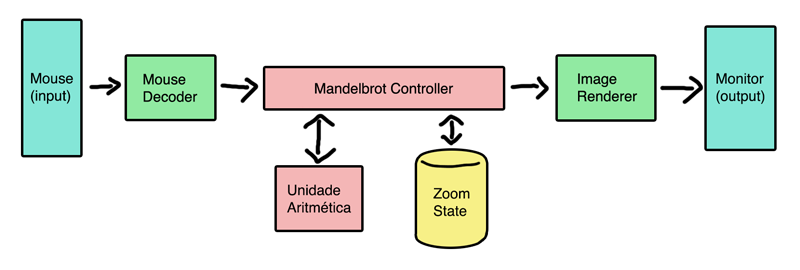
\includegraphics[width=1\textwidth]{./block_diagram.png}~\\[2cm]

Mouse Decoder : interpreta o mouse

Mandelbrot Controller : controla as iterações na criação do conjunto de Mandelbrot

Unidade Aritmética : realiza as operações aritméticas com os números complexos

Zoom State : armazena o quão ampliado está a imagem e a região que está sendo exibida

Image Renderer : traduz os pontos para uma imagem

\section{Descrição do Sistema Implementado}
Todo o sistema foi implementado com o auxílio da biblioteca "numeric\_std" e "fixed\_pkg", que auxiliaram para a utilização de números inteiros e de ponto fixo. No total foram usados 7 módulos:\\

\subsection{fractal}
É o top level que conecta os outros componentes do projeto.\\
\subsection{control}
Maquina de estados que controla os outros componentes do projeto.\\
-o primeiro estado é somente responsável por inicializar as variáveis.\\
-o segundo estado calcula para cada pixel qual seria seu equivalente no plano complexo e salva nas memórias constMem.\\
-o terceiro estado envia as constantes complexas das constMems para iterar na função de Mandelbrot e salvar na SRAM.\\
-o quarto estado espera um comando do usuário.\\
\subsection{constMem}
São 2 memórias RAMS(uma para x e outra para y) com portas de entrada e de saída, criadas com o software Quartus. A porta de entrada é usada no segundo estado de "Control", quando ele escreve as constantes nas memórias, a de saída é usada no terceiro estado, quando ele envia essas constantes para iterar na função de Mandelbrot.\\
\subsection{mandelbrot}
Recebe duas constantes x e y(ou seja o ponto $z = x + iy$) e itera 65 vezes(esse foi o número que apresentou resultados mais satisfatórios, números maiores podem corromper a imagem ou atrasar desnecessariamente o cálculo da renderização) na função de Mandelbrot. Tem duas saídas, uma que diz se terminou as iterações e outra que indica se alguma vez o módulo do ponto passou de 2.
\subsection{memory\_control}
Escreve e Lê os pontos calculados pelo "mandelbrot" na memória SRAM. Esses pontos são passados como parâmentro para o componente "VGA". Um detalhe que deve ser mencionado é que - devido a limitações de espaço - ao invés de se usar toda a palavra da SRAM para cada pixel usamos apenas metade, fazendo usos dos pinos "SRAM\_UB\_N" e "SRAM\_LB\_N".
\subsection{VGA}
Esse componente gera os sinais de sincronia e imprime a imagem na tela.

Como especificado anteriormente, a resolução utilizada foi de 640x480 com 60Hz de frequência, com o auxílio do site \url{http://www.epanorama.net/faq/vga2rgb/calc.html}, foi possível calcular o Front Porch, Sync Pulse e Back Porch dos sinais de sincronia.\\ Para o sinal horizontal(VGA\_HS):\\
FP = 24\\
SP = 40\\
BP = 128\\
Já para o sinal vertical(VGA\_VS):\\
FP = 9\\
SP = 3\\
BP = 28\\

\section{Conclusões}
Por diversas razões, esse projeto foi mais desafiador do que o grupo esperava: a necessidade de ter que primeiro salvar os pontos numa memória(constMem), utilizar a SRAM utilizando as flags de palavra alta e palavra baixa, escrever um próprio componente "VGA" pois a resolução não estava funcionando no componente "vgacon" disponibilizado, e por fim, as iterações do mandelbrot consumirem bastante tempo, foram alguns dos empecilhos para o desenvolvimento do projeto.\\
Por outro lado, essas adversidades contribuíram para que o grupo desenvolvesse sua capacidade de programar hardware e entendesse melhor o funcionamento da placa.\\

\section{Comentários e Sugestões}
Algumas mudanças podem ser facilmente implementadas para tornar o projeto ainda mais interessante.\\
\subsection{Pintar de Diferentes Cores}
Poderíamos, por exemplo, ao invés de "pintar" de preto ou branco, pintar de cores graduais dependendo do número de iterações necessárias para o ponto escapar. A figura a seguir ilustra uma possibilidade dessa abordagem.\\[1cm]


\includegraphics[width=0.6\textwidth]{./Mandelbrot-Color.png}~\\[2cm]
\subsection{Conjuntos de Julia}
Fazendo uma alteração simples na fórmula de iteração podemos criar padrões igualmente interessantes: se colocarmos o número complexo $z_p$ equivalente ao pixel $p$ como sendo o valor inicial de $z_0$, e definirmos $c$ como uma constante arbitrária, criamos padrões fractais conhecidos como o conjuntos de Julia(em homenagem ao matemático Gaston Julia). A fórmula então seria:
$$ z_0 = z_p$$
$$z_{n+1} = {z_n}^2 + c$$
\\[4cm]
Para $c = -0.74434 -0.10772i$ por exemplo, temos o seguinte fractal:\\[1cm]

\includegraphics[width=0.8\textwidth]{./julia.png}

\section{Fotos do Projeto}
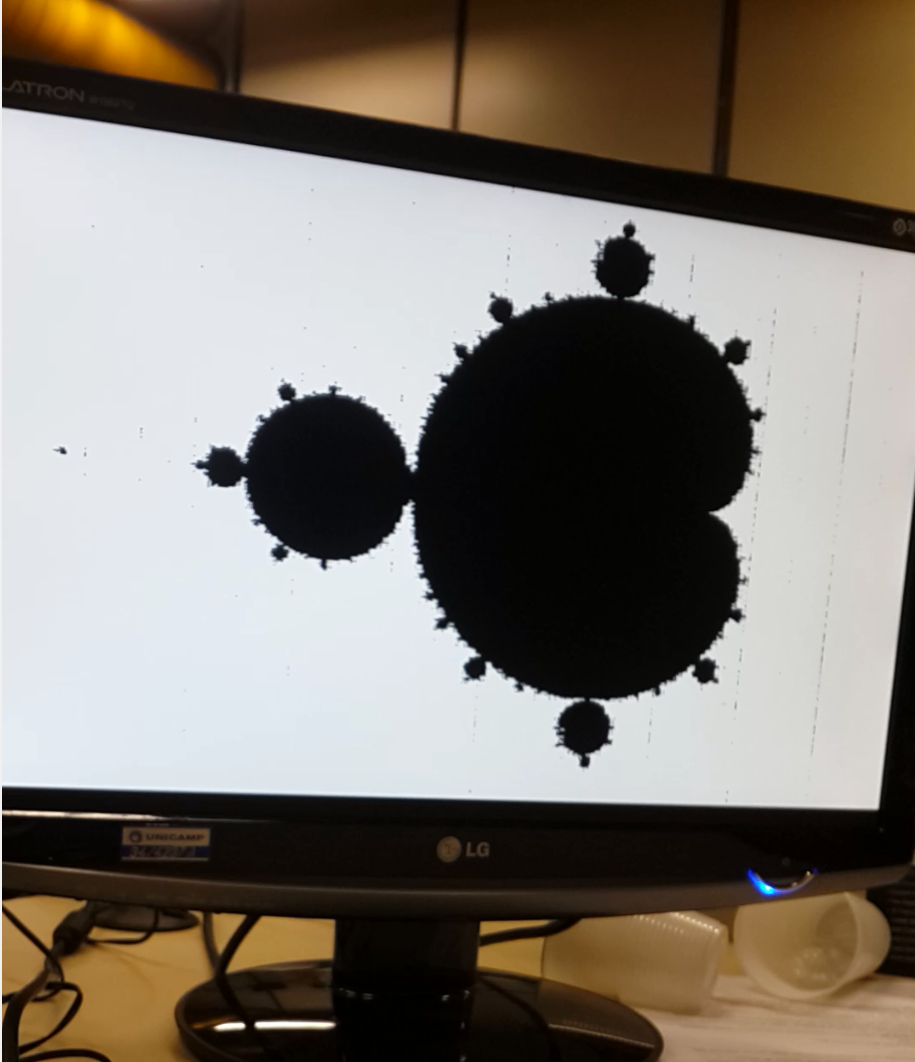
\includegraphics[width=0.4\textwidth]{./imagem1.png}
\ \  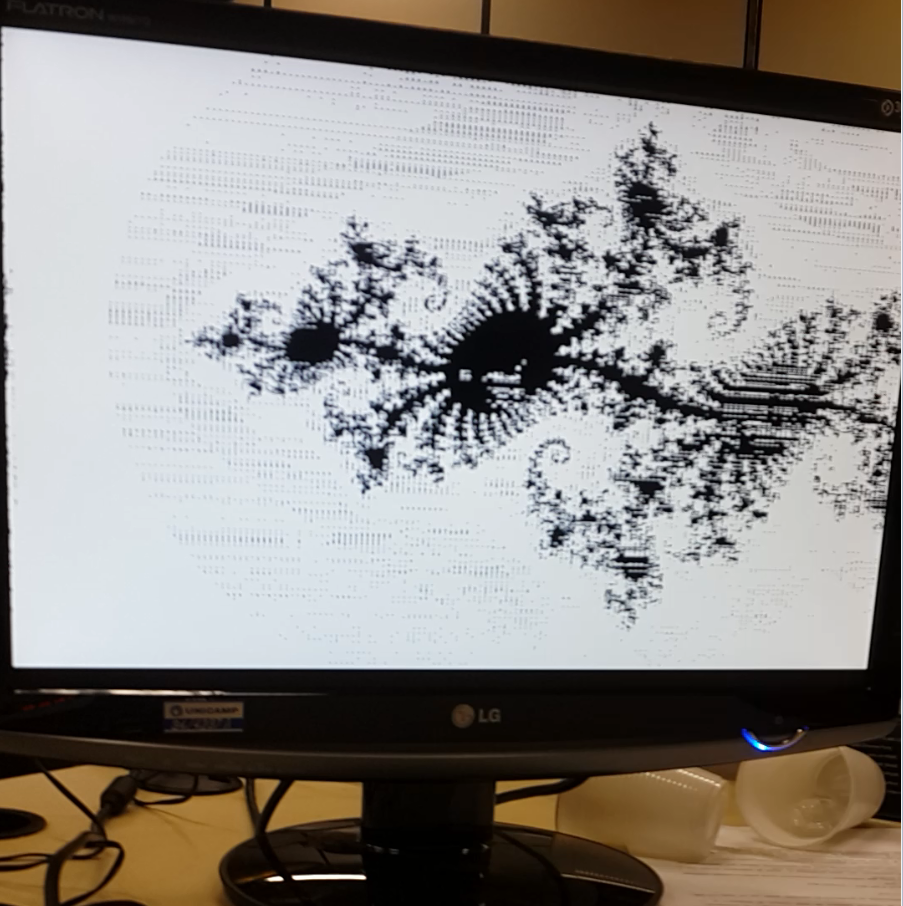
\includegraphics[width=0.5\textwidth]{./imagem2.png}\\[1cm]

\section{Referências}
\url{http://www.ic.unicamp.br/~cortes/mc613/}\\
\url{https://en.wikipedia.org/wiki/Mandelbrot_set}\\
\url{http://webserv.jcu.edu/math//vignettes/Julia.htm}\\
\url{https://github.com/imr/Mandelbrot-VHDL}
\end{document}